\section{Results}
Search times over filesizes were times for queries of all depths ranging from depth 1 to depth 7. All these plots can be found in the appendix. Figure \ref{fig:Searchtimebool1} shows the search time for 1000 randomly generated queries of depth 1. For clarification, a depth of 1 means the act of either inverting one article list for a given word or using the AND or the OR operation on two article lists for two given words.

\begin{figure}[ht!]
    \centering
    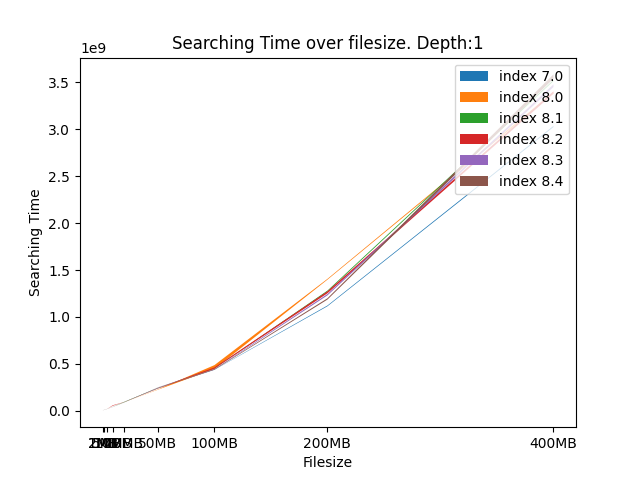
\includegraphics[width=.8\textwidth]{LaTeX/Pictures/Results/BooleanSearchDepth0.png}
    \caption{Search times for the Boolean queries of depth 1 of index 7.0, 8.0, 8.1, 8.2, 8.3 and 8.4. The time on the y-axis is measured in $ns$}
    \label{fig:Searchtimebool1}
\end{figure}

Figure\ref{fig:Searchtimebool7} shows the search time for 1000 randomly generated queries of depth 7.

\begin{figure}[ht!]
    \centering
    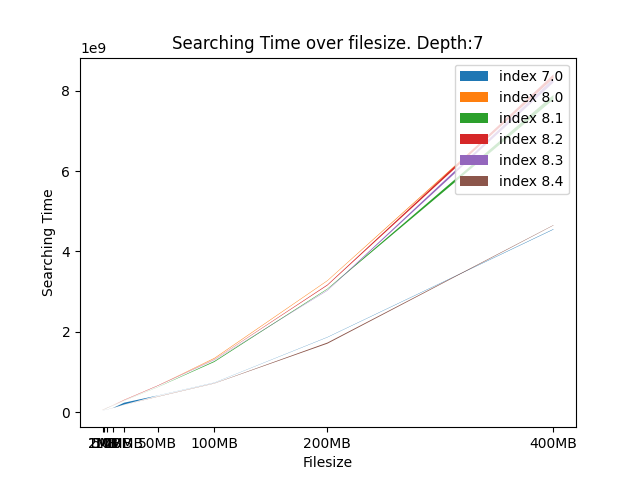
\includegraphics[width=.8\textwidth]{LaTeX/Pictures/Results/BooleanSearchDepth6.png}
    \caption{Search times for the Boolean queries of depth 7 of index 7.0, 8.0, 8.1, 8.2, 8.3 and 8.4. The time on the y-axis is measured in $ns$}
    \label{fig:Searchtimebool7}
\end{figure}

Figure\ref{fig:IndexingBool} shows the indexing time for the Boolean indices.

\begin{figure}[ht!]
    \centering
    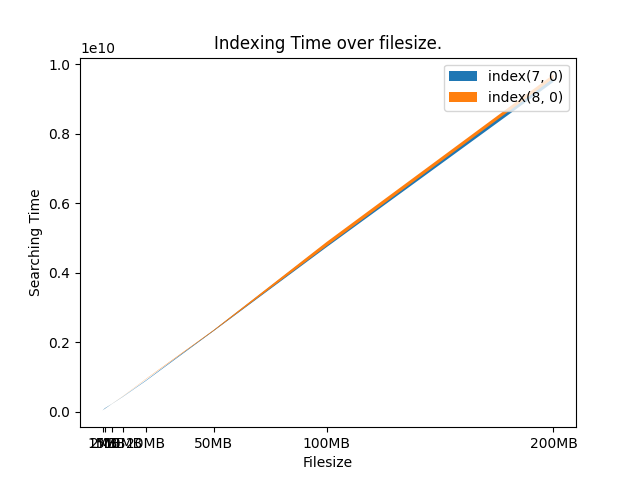
\includegraphics[width=.8\textwidth]{LaTeX/Pictures/Results/Indexing[(7, 0), (8, 0)].png}
    \caption{Indexing times for index 7 and 8. The time on the y-axis is measured in $ns$}
    \label{fig:IndexingBool}
\end{figure}